\documentclass{handout}
\usepackage{handoutSetup}\usepackage{handoutShortcuts}
 

\begin{document}
\handoutHeader

\begin{verbatimwrite}{\jobname.title}
The Diamond (1965) OLG Model
\end{verbatimwrite}

\handoutNameMake

This handout and the associated Jupyter notebook, \href{https://econ-ark.org/materials/diamondolg?launch}{DiamondOLG}, present a canonical overlapping generations (OLG) model, like the one originally proposed by \cite{diamond:olg}, building on \cite{samuelson:olg}.\footnote{For a remarkably clear statement of the questions addressed by OLG models, see \cite{jeffersonOLG}.  For a review of the influence of \cite{samuelson:olg}'s model, see \cite{weilSamuelson}.}

\section{Setup}

The economy has the following features:
\begin{enumerate}

\item Two generations are alive at any point in time, the young (age 1) and old (age 2).

\item The size of the {\it young} generation in period $t$ is given by \opt{MarginNotes}{\marginpar{\tiny Note that $\PopLev$ is not whole pop - just young.}}
$\PopLev_{t}=\PopLev_{0}\PopGro^{t}$.\opt{MarginNotes}{\marginpar{\tiny That is, constant pop growth since time 0.}}

\item Households work only in the first period of life, earning income $Y_{1,t}$.  They
earn no income in the second period of life ($Y_{2,t+1}=0$).

\item They consume part of their first-period income and save the rest to finance their 
consumption when old.

\item The assets of the young at the end of period $t$ are the source of the 
capital used for aggregate production in period $t+1$, $\KLev_{t+1} = 
\PopLev_{t}{\aLev}_{1,t}$ where ${\aLev}_{1,t}$ is the assets per young household {\it after} their
consumption in period 1.  (For convenience, we assume that there is no depreciation).  \opt{MarginNotes}{\marginpar{\tiny First example of convention that will be used repeatedly in this class: lower-case letter is per-capita.}}

\item \opt{MarginNotes}{\marginpar{\tiny Point out that it's $\PopLev_{t-1}$ b/c old in $t$ were young in $t-1$ and $\PopLev_{t-1}$ is size of pop of young in $t-1$.}}  The old in period $t$ own the entire capital stock and (because they have 
no bequest motive) will consume it all, so dissaving by the old in 
period $t$ will be $\PopLev_{t-1}{\aLev}_{1,t-1} = \KLev_{t}$.  (The old do receive
interest on their capital, so their consumption will be $\KLev_{t}$ plus
the interest income $\rfree \KLev_{t}$, but the $\rfree \KLev_{t}$ component does not 
affect saving because it is part of both income and consumption).

\item Labor and capital markets are perfectly
competitive and the aggregate production technology is CRS, $\YLev=\FFunc(\KLev,\LLev)$
(recall that this implies that $\FFunc(\KLev,\LLev) = \FFunc_{L}\LLev + \FFunc_{K}\KLev$,
which is \href{https://www.econ2.jhu.edu/people/ccarroll/public/LectureNotes/MathFacts/MathFactsList/#EulersTheorem}{``Euler's Theorem''}.

\end{enumerate}

\section{Analysis}

Let's normalize everything by the period-$t$ young population $\PopLev_{t}$, 
writing normalized variables in lower case.  Thus the per-young-capita 
aggregate production function becomes 
\begin{equation}
        \fFunc(\kLev_{t}) \equiv \FFunc(\KLev_{t},\PopLev_{t})/\PopLev_{t} = \FFunc(\KLev_{t}/\PopLev_{t},1). \label{eq:fFromF}
\end{equation}

The perfect competition assumption implies that wages and net interest 
rates are equal to the marginal products of labor and capital, 
respectively: 
\begin{equation}\begin{gathered}\begin{aligned}
        \Wage_{t} & =  \fFunc(\kLev_{t}) - \kLev_{t}\fFunc^{\prime}(\kLev_{t}),
\\      \rfree_{t} & =  \fFunc^{\prime}(\kLev_{t}) \label{eq:rEqfp}.
\end{aligned}\end{gathered}\end{equation}

To make further progress, we need to make specific assumptions about 
the utility function and the aggregate production function.  Assume 
that utility is CRRA, $\uFunc(\bullet) = \bullet^{1-\CRRA}/(1-\CRRA)$ and assume a 
Cobb-Douglas aggregate production function $\FFunc(\KLev,\LLev) = \KLev^{\varepsilon}\LLev^{1-\varepsilon} \Rightarrow \fFunc(\kLev) = \kLev^{\varepsilon}$.

In this case we can solve for wages and interest rates:
\begin{equation}\begin{gathered}\begin{aligned}
        \Wage_{t} & =  (1-\varepsilon) \kLev^{\varepsilon}_{t}  \\
        \rfree_{t} & =  \varepsilon \kLev^{\varepsilon-1}_{t}.
\end{aligned}\end{gathered}\end{equation}

The individual's maximization problem yields the Euler equation:\opt{MarginNotes}{\marginpar{\tiny Recall that $R=1+r$, an example where lower-case does not signify per-capita.}}
\begin{equation}
\uFunc^{\prime}(\cLev_{1,t}) = \Discount \Rfree_{t+1} \uFunc^{\prime}(\cLev_{2,t+1}). 
\end{equation}

Now let's assume that utility is logarithmic, $\CRRA = 1$, which implies that \opt{MarginNotes}{\marginpar{\tiny Begin with consumption in levels, not per-capita, and move to per-capita in \eqref{eq:cratio}}}{}
\begin{equation}\begin{gathered}\begin{aligned}
        \cLev_{1,t} & =  \frac{\Wage_{1,t} + \overbrace{\Wage_{2,t+1}}^{=0}/\Rfree_{t+1}}{1+\Discount}  \\
        \cLev_{1,t} & =  \frac{\Wage_{1,t}}{1+\Discount} \\
        {\aLev}_{1,t} & =  \Wage_{1,t}-\cLev_{1,t}  \\
         & =  \Wage_{1,t}(1-1/(1+\Discount))  \\
         & =  \Wage_{1,t}(\Discount/(1+\Discount))
\\   & =  (1-\varepsilon) \kLev_{t}^{\varepsilon}\left(\frac{\Discount}{1+\Discount}\right)
\\  \overbrace{\kLev_{t+1}}^{={\aLev}_{1,t}/\PopGro} & =  \kLev_{t}^{\varepsilon}\left[\frac{(1-\varepsilon)\Discount}{\PopGro(1+\Discount)}\right] \label{eq:ktp1}
\\ \frac{d\kLev_{t+1}}{d\kLev_{t}} & =  \kLev_{t}^{\varepsilon-1}\left[\frac{\varepsilon (1-\varepsilon) \Discount}{\PopGro(1+\Discount)}\right].
\end{aligned}\end{gathered}\end{equation}

The steady-state will be the point where $\kLev_{t+1}=\kLev_{t}$.  For convenience,
define a constant
\[ \mathcal{Q} = \frac{(1-\varepsilon) \Discount}{\PopGro(1+\Discount)}, \]
allowing us to rewrite \eqref{eq:ktp1} as
\begin{equation}\begin{gathered}\begin{aligned}
        \kLev_{t+1} & =  \mathcal{Q} \kLev_{t}^{\varepsilon}.
\end{aligned}\end{gathered}\end{equation}

Then the steady-state will be the point where $\kLev_{t+1}=\kLev_{t}=\bar{\kLev}$
\begin{equation}\begin{gathered}\begin{aligned}
        \bar{\kLev} & =  \mathcal{Q} \bar{\kLev}^{\varepsilon}  \\
        \bar{\kLev} & =  \mathcal{Q}^{1/(1-\varepsilon)}.
\end{aligned}\end{gathered}\end{equation}

Dynamics of the model can be analyzed using a simple figure relating 
the capital stock per capita in period $t+1$ to that in period $t$.  
The solid locus is a graph of equation \eqref{eq:ktp1}.  We depict the 
45 degree line because it indicates the set of `steady-state' points 
where $\kLev_{t+1}=\kLev_{t}$ and thus any intersection of the 45 degree line 
with the $\kLev_{t+1}(\kLev_{t})$ function indicates a steady-state of the 
model.

\begin{figure}
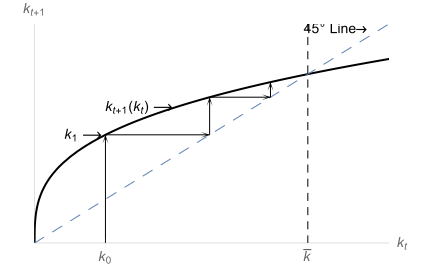
\includegraphics[width=6in]{Figures/OLGModelDynamics}
\caption{Convergence of OLG Economy to Steady State}
\label{fig:OLGModelDynamics}
\end{figure}

The experiment traced out in the figure is as follows.  We start the 
economy in period $t=0$ with capital per capita of $\kLev_{0}$, which, 
from \eqref{eq:ktp1}, implies a certain value $\kLev_{1}$ for capital in 
period $t+1=1$.  Now think about period $1$ becoming $t$ and period 
$2$ becoming $t+1$.  To find the correct level of capital implied by 
the model in period $t+2$ we need to find the point on the 45 degree 
line that corresponds to $\kLev_{1}$, then go vertically up from there to 
find $\kLev_{t+1}=\kLev_{2}$.  When the same set of gyrations is repeated the 
result is that the level of capital converges to the steady-state 
level $\bar{\kLev}$.

\section{Social Optimum}

We have determined the outcome that will arise in a perfectly 
competitive economy in which households optimally choose their
behavior given market prices with no government intervention.

Often in macroeconomic analysis this constellation of assumptions
yields a conclusion that the steady state is optimal (and dynamics are also optimal)
according to some plausible criteria.  We now examine the optimality
properties of the OLG model outcome.

As a preliminary, let's define the lifetime utility experienced 
by the young generation at time $t$ as
\begin{equation}\begin{gathered}\begin{aligned}
  \label{eq:lifeUtil}
  \vFunc_{t} & =  \uFunc(\cLev_{1,t})+\Discount \uFunc(\cLev_{2,t+1})
.
\end{aligned}\end{gathered}\end{equation}

Suppose our definition of optimality reflects the choices that would
be made by a benevolent social planner who maximizes a social
welfare function of the form\footnote{The $\Discount$ multiplying the level of utility for the old generation at time $t$ is necessary to prevent the social planner's problem from exhibiting time inconsistency.}
\begin{equation}\begin{gathered}\begin{aligned}
  \VFunc_{t} & =  \Discount \uFunc(\cLev_{2,t}) + \sum_{n=0}^{\infty} \beth^{n} \vFunc_{t+n}
\end{aligned}\end{gathered}\end{equation}
subject to the economy's aggregate resource constraint
\begin{equation}\begin{gathered}\begin{aligned}
  \label{eq:Bud}
  \underbrace{\KLev_{t} + \FFunc(\KLev_{t},\PopLev_{t})}_{\text{Sources}} & =  \underbrace{\KLev_{t+1} + \PopLev_{t} \cLev_{1,t} + \PopLev_{t-1} \cLev_{2,t}}_{\text{Uses}}
\end{aligned}\end{gathered}\end{equation}
where the Hebrew letter $\beth$ reflects the social planner's discount factor
and the planner must allocate the society's resources (``Sources'') between
consumption of the two generations alive at time $t$ and the capital stock
in period $t+1$ (``Uses'').  

The idea is that the social planner cares about every generation's lifetime happiness,
but discounts the happiness of future generations.  (We will discuss why discounting
is necessary later in the class).


It is possible to show (using methods not described in this handout; see~\cite{blanchard&fischer:text} for details) that the socially optimal steady state is 
characterized by the equation
\begin{equation}\begin{gathered}\begin{aligned}
  1+\fFunc^{\prime}(\bar{\kLev}^{*}) & =  \PopGro \beth^{-1}
\end{aligned}\end{gathered}\end{equation}

In the case of our Cobb-Douglas production function, this 
becomes
\begin{equation}\begin{gathered}\begin{aligned}
  \label{eq:2}
  (\bar{\kLev}^{*})^{\varepsilon-1}\varepsilon  & =  \PopGro \beth^{-1} - 1
\\ \bar{\kLev}^{*} & =  \left(\frac{\PopGro \beth^{-1} - 1}{\varepsilon}\right)^{1/(\varepsilon-1)}
.
\end{aligned}\end{gathered}\end{equation}

Comparing this to the outcome that will actually arise, 
\begin{equation}\begin{gathered}\begin{aligned}
\bar{\kLev} & =  \left(\frac{\PopGro(1+\Discount)}{(1-\varepsilon) \Discount}\right)^{1/(\varepsilon-1)},  
\end{aligned}\end{gathered}\end{equation}
our point is that there is no particular relationship between
the socially optimal outcome and the actual equilibrium outcome
that will arise if the social planner is not involved.  The actual
outcome could have too little capital or too much, and there is no 
reason to expect it to be the ``right'' amount.

You might respond by saying that our definition of optimality here
is too strong; we might hope that the economy would at least be able
to avoid a Pareto inefficient outcome, even if we can't expect 
perfect optimality according to the preferences of some mythical Godlike 
``social planner.''

It turns out, however, that even Pareto efficiency is not guaranteed.
(In this context, Pareto efficiency must be defined across generations:
The economy is Pareto efficient if there is no way to make one generation
better off without making another generation worse off).

To examine Pareto efficiency, start by rewriting the aggregate DBC by
dividing by the size of the labor force at time $t$:
\begin{equation}\begin{gathered}\begin{aligned}
  \label{eq:5}
  \kLev_{t} + \fFunc(\kLev_{t}) & =  \PopGro \kLev_{t+1} + \cLev_{1,t} + \cLev_{2,t}/\PopGro
\end{aligned}\end{gathered}\end{equation}

Define an index of aggregate per capita consumption as 
\begin{equation}\begin{gathered}\begin{aligned}
  \label{eq:6}
  \cLev_{t} & =  \cLev_{1,t} + \cLev_{2,t}/\PopGro
\end{aligned}\end{gathered}\end{equation}

In steady state, $\kLev_{t+1}=\kLev_{t}=\bar{\kLev}$, so if $\bar{\cLev}$ is the steady-state level of 
$\cLev_{t}$ then the accumulation equation
implies
\begin{equation}\begin{gathered}\begin{aligned}
  \bar{\kLev} + \fFunc(\bar{\kLev}) & =  \PopGro \bar{\kLev} + \bar{\cLev}
\\ \fFunc(\bar{\kLev}) & =  \underbrace{(\PopGro-1)}_{\popGro}\bar{\kLev}+\bar{\cLev}
\\ \fFunc(\bar{\kLev})-\popGro \bar{\kLev} & =  \bar{\cLev}
\end{aligned}\end{gathered}\end{equation}

Now consider the effects of a change in $\bar{\kLev}$ on $\bar{\cLev}$:
\begin{equation}\begin{gathered}\begin{aligned}
  \left(\frac{d \bar{\cLev}}{d \bar{\kLev}}\right) & =  \fFunc^{\prime}(\bar{\kLev})-\popGro.
\end{aligned}\end{gathered}\end{equation}

There exists a $\bar{\kLev}$ which maximizes per-capita
steady-state consumption:
\begin{equation}\begin{gathered}\begin{aligned}
  \max_{\bar{\kLev}} ~ \fFunc(\bar{\kLev}) - \popGro \bar{\kLev}
\end{aligned}\end{gathered}\end{equation}
whose solution is obtained from the FOC
\begin{equation}\begin{gathered}\begin{aligned}
  \varepsilon \bar{\kLev}^{\varepsilon-1} & =  \popGro
\\ \bar{\kLev}^{**} & =  (\popGro/\varepsilon)^{1/(\varepsilon-1)},
\end{aligned}\end{gathered}\end{equation}
and note that this means that for $\bar{\kLev} \geq \bar{\kLev}^{**}$ 
an extra bit of capital actually requires a {\it decline} in 
steady-state consumption.  An economy in this circumstance of 
excessive saving is called `dynamically inefficient.'

Note further that there is actually a $\bar{\kLev}$ so large that
consumption would have to be zero:
\begin{equation}\begin{gathered}\begin{aligned}
  \bar{\kLev}^{\varepsilon} & =  \popGro k
\\ \bar{\kLev}^{\varepsilon-1} & =  \popGro
\\ \bar{\kLev} & =  \popGro^{1/(\varepsilon-1)}.
\end{aligned}\end{gathered}\end{equation}

These points are illustrated graphically in the remaining figure.

\begin{figure}
\caption{Gross and Net Per Capita Output as a Function of $\kLev$}
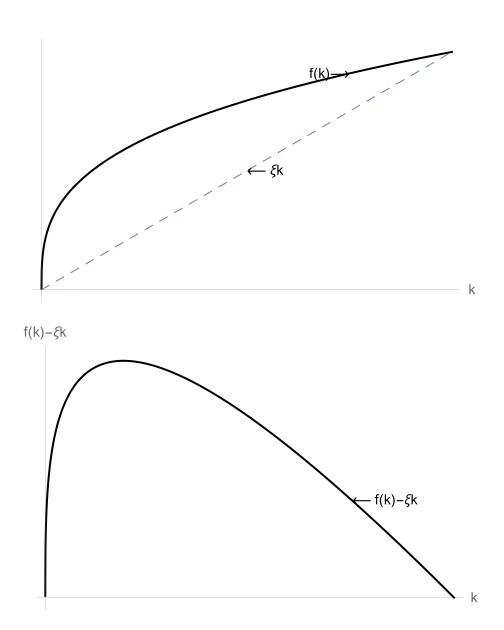
\includegraphics[width=6in]{Figures/fnkBoth}
\end{figure}

\pagebreak
\input handoutBibMake.tex
 

\end{document}
